\documentclass{article}

\usepackage[solutions]{xrcise}

\begin{document}
\sheet[2012]{Ersttermin}

\begin{exercise}{Multiple Choice}
  \begin{enumerate}
    \item
  \end{enumerate}
  %   Bei allen Multiple-Choice Fragen ist genau ein Kreuz zu setzen. Sollte mehr als ein Kreuz gesetzt sein, wird die Teilaufgabe mit 0 Punkten gewertet.
  % 1. Gegeben sind die Funktionen
  % n2 n! n2n √3 n Welche der folgenden Aussagen gilt?
  % Alle Funktionen sind polynomiell.
  % n! ist die am stärksten wachsende Funktion √3 n = O(log(n))
  % n2 + o(n2) = Θ(n2)
  % log(n)
  % 2. Seien f (n), g(n) Funktionen. Weiter sei h definiert durch h(n) = max(f (n), g(n)). Gilt dann (2 Punkte)
  % h(n) = O(f(n))
  % h(n) = O(f (n) + g(n)) h(n) = ω(f (n) + g(n)) h(n) = O(f (n) − g(n))
  % 3. Beschreiben Sie die Datenstruktur Schlange, die sich durch die folgende Sequenz von Operationen ergibt: (1 Punkt)
  % enqueue(15), rear(), enqueue(7), enqueue(8), dequeue(), enqueue(9), de- queue(), head(), enqueue(10)
  % 4. Wir betrachten einen Baum T mit Höhe h (die Wurzel hat die Höhe 0) und n Kno- ten. Die inneren Knoten von T haben maximal drei Kinder. Welche der folgenden
  % Aussagen ist wahr?
  % h ist immer log3(n)
  % T hat mindestens n Kanten
  % T hat immer mehr Blätter als innere Knoten T hat mindestens n − 3h innere Knoten.
  % Sei G = (V,E) ein zusammenhängender, ungerichteter Graph mit der Kanten- gewichtsfunktion w. Angenommen w(e) = c, c konstant, für alle Kanten, welche Laufzeit lässt sich dann zur Berechnung des minimalen Spannbaumes in G errei- chen? (2 Punkte)
  % O(|V | log |E|) O(|V | + |E|) O(|E| log |V |) O(|V |2)
  % 6. Fügen Sie den Wert 12 in die folgende Hashtabelle mit offener Addressierung und linearer Sondierung ein. Als Hashfunktion wird h(x) = x mod 7 benutzt.
  % 0123456
  % 9 513 7. Führen Sie eine Linksrotation auf den Knoten a aus.
  % e ag
  % cfh bd
  % LEFT-ROTATE(a)
  % 8. Seien L, L′ ∈ P . Welche der folgenden Aussagen ist falsch? Wenn L ∈ NP gilt, dann folgt P = NP
  % ∀L′′ ∈NPC:L≤p L′′
  % L ∩ L′ ∈ P
  % L ∪ L′ ∈ P
  % Welches ist die untere Schranke für die Anzahl der Vergleichsoperationen bei ver-
  % gleichsbasierten Sortieralgorithmen?
  % Ω(n) Ω(log(n))
  % Ω(n log(n)) Ω(n2 )
  % 10. In einem minimalen Spannbaum eines Graphen mit n Knoten
  % kann die Kante mit dem höchsten Gewicht enthalten sein
  % darf die Kante mit dem kleinsten Gewicht nicht enthalten sein können mehr als n − 1 Kanten enthalten sein
  % muss die Summe der Kantengewichte durch 2 teilbar sein
  % (2 Punkte)
  % (2 Punkte)
  % 11. In einem Rot-Schwarz-Baum gilt (ohne Betrachtung der Wächter) für alle roten Knoten r (2 Punkte)
  % der Vor-Vorgänger von r ist rot, falls der Elter von r nicht die Wurzel ist der Bruder Knoten von r ist rot
  % Wenn r kein Blatt ist, dann hat r zwei Kinder
  % der Onkel von r ist schwarz

  \begin{solution}

  \end{solution}
\end{exercise}

\begin{exercise}{Algorithmenanalyse}
  \begin{enumerate}
    \item
          %     Betrachten Sie die folgenden Code-Segmente. Geben Sie für jedes Segment eine möglichst dichte Schranke für die asymptotische Laufzeit im O-Kalkül in Abhän- gigkeit von N, bzw. N = length[A] an. Bei rekursiven Algorithmen formulieren Sie zuvor die Rekurrenzgleichung. (Teil-Arrays werden immer als Kopie übergeben, das
          % Kopieren kostet keine Zeit.)
          % Alg1()
          % for i = 0 to N
          % doforj←N downto1
          % (14 Punkte)
          % O( )
          % O( )
          % O( )
          % 
          % Alg2()
          % do
          % sum ← sum + j
          % > 1
          % sum ← sum + j j ← j/2
          % for i = 1 to N do j←N
          % while j do
          % Alg3()
          % while N >1
          % do for j ← 1 to N
          % do sum ← sum + j N ← N/2
          % Alg4(A)
          % middle ← length[A]/2
          % sum ← sum + A[1] if length[A] > 2
          % then Alg4(A[1 . . middle]) Alg4(A[middle + 1 . . length[A]])
          % Alg5(A)
          % for i ← 1 to length[A]
          % do sum ← sum + A[i]2
          % T(N) = 
          % O( )
          % if length[A] > 3
          % then Alg5(A[1 . . length[A]/3]) O(
          % Alg5(A[length[A]/3 . . 2 · length[A]/3]) Alg5(A[2 · length[A]/3 . . length[A]])
          % Alg6(A)
          % for i ← 1 to length[A]
          % do sum ← sum + A[i]
          %  
          % T(N) = 
          % if length[A] > 1 O( then Alg6(A[1 . . length[A] − 2])
          % Alg7(A)
          % sum ← sum + 1 if length[A] > 1
          % )
          % )
          % then Alg7(A[1 . . length[A] − 2]) O( Alg7(A[2 . . length[A] − 1])
    \item
          % Bestimmen Sie die asymptotische Laufzeit des folgenden Algorithmus mit der Sub-
          % stitutionsmethode, geben Sie Ihren Lösungsweg an:
          % Alg8(A, N, n)
          % if n ≥ 2
          % then for i ← 1 to n
          % do swap(A[i], A[r]) Alg8(A, N, n − 1) swap(A[r], A[i])
          % else sum ← 0
          % for i ← 1 to N
          % do s ← s+A[i]
          % Die Funktion wird aufgerufen mit: Alg8(A, length[A], length[A])
          % Hinweise:
          % (6 Punkte)
          % a) VerwendenSiefolgendeNotation:[n]i =n·(n−1)·...·(n−i)
          % b) Verwenden Sie die Abschätzung [n]i ≤ n!, wenn dies nicht zu einer Erhöhung
          % der Laufzeitschranke im O-Kalkül führt.
  \end{enumerate}

  \begin{solution}

  \end{solution}
\end{exercise}

\begin{exercise}{Quicksort}
  %   Gegeben sei die bekannte Partitionsfunktion aus dem Quicksort-Algorithmus
  % Partition(A, l, r)
  % 1 2 3 4 5 6 7 8
  %  l - linkes Blockende, r - rechtes Blockende, A[r] - Pivot i←l−1
  % forj←ltor−1
  % do if A[j] ≤ A[r] then i ← i + 1
  % SWAP(A[i], A[j]) SWAP(A[i + 1], A[r])
  % return (i + 1)
  % Dabei gehen wir in dieser Aufgabe von Arrays mit 0-basiertem Index aus. Sie befinden sich in Zeile 4 der Partition-Funktion mit l = 0,r = 6 und j = 3,i = 0. Werten Sie alle Schritte bis zum Erreichen der Zeile 8 aus. Protokollieren Sie den
  % Speicherzustand jeweils beim Erreichen der Zeile 4 und der Zeile 8.
  % Zeile4,A: 3 Zeile 4, A: Zeile 4, A: Zeile 8, A:
  % 8 6 4
  % 6 4 5
  % j=3,i=0 j = 4, i =
  % j = 5, i =
  % j = 5, i =

  % Ist Quicksort mit der obigen Partition Funktion ein stabiles Sortierverfahren? Begründen Sie Ihre Antwort und zeigen Sie entweder, dass Partition stabil ist oder schlagen Sie eine Modifikation von Quicksort vor, welche diesen stabilisiert.

  % Gegeben sei ein Array der Länge N, welches ausschließlich Elemente aus der Menge 0,1,2 enthält. Entwerfen Sie einen Algorithmus, der die Elemente in O(n) Zeit sortiert. Der Algorithmus soll vergleichs-/austauschbasiert und in-place arbeiten, was bedeutet, dass er maximal O(1) zusätzlichen Speicher nutzen darf. Skizzieren Sie Ihre Idee mit Pseudo-Code und einem beschreibenden Text.
  \begin{solution}

  \end{solution}
\end{exercise}

\begin{exercise}{Minimaler Spannbaum}
  \begin{figure}
  \centering

  \caption{A graph}\label{fig:mstgraphrarey}
\end{figure}
  % Zeichnen Sie in den oben angegebenen Graphen einen minimalen Spannbaum ein. Ist dieser Spannbaum eindeutig? Begründen Sie Ihre Antwort.

  % Gegeben sei ein Graph G = (V,E). Entwerfen Sie einen rekursiven Algorithmus Label(V, E, u, ’label’), der einen Knoten u und alle von u aus erreichbaren Knoten mit der Markierung ’label’ versieht. Der Algorithmus soll die Laufzeit O(|V | + |E|) haben. Beschreiben Sie Ihren Algorithmus und geben Sie Pseudo-Code für die
  % Funktion Label an.

  % In einem Graphen G = (V,E) mit Kantengewichten bezeichnen wir eine Kante e eines minimalen Spannbaums T als kritisch, wenn das Entfernen von e das Gewicht des minimalen Spannbaums in G vergrößert. Entwickeln Sie einen Algorithmus, der in O(|V | + |E|) Zeit entscheidet, ob e kritisch ist. Nutzen Sie dabei die Funktion Label aus der vorausgehenden Aufgabe als Hilfsfunktion. Beschreiben Sie kurz Ihren Lösungsweg und geben Sie den Algorithmus im Pseudo-Code an. Argumen- tieren Sie außerdem in wenigen Stichpunkten, warum Ihr Algorithmus korrekt ist.
  \begin{solution}

  \end{solution}
\end{exercise}

\begin{exercise}{Graphen}
  \begin{figure}
  \centering
  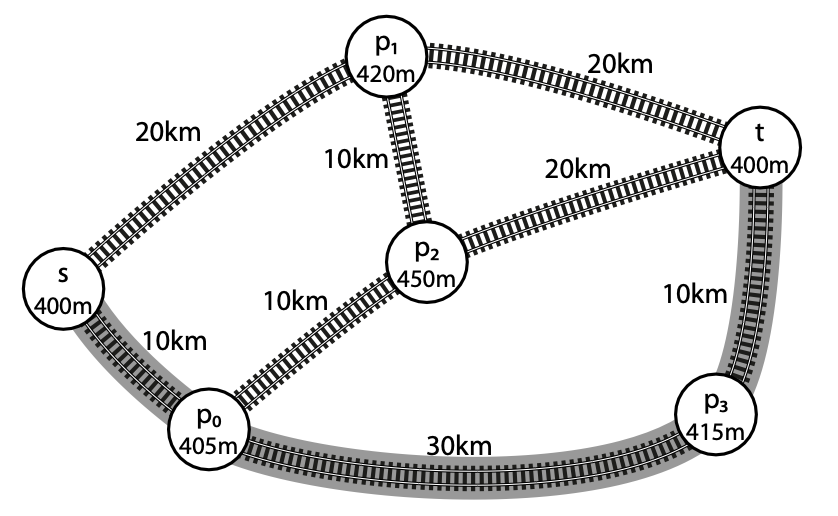
\includegraphics{res/trains.png}
  \caption{Train line graph.}\label{fig:trains}
\end{figure}
  %   Eine neue Eisenbahnlinie soll gebaut
  % werden und Sie wurden mit ihrer Pla-
  % nung beauftragt. Zur Verfügung steht 20km 10km
  % Ihnen eine topographische Landkarte
  % mit möglichen Streckenverlaufspunk-
  % ten pi. Auf der Karte sind die Distan- s
  % zen in km zwischen den Punkten ein- 400m
  % getragen sowie die Höhe der Strecken-
  % verlaufspunkte über Normalnull in Me- p0
  % tern. Ihr Auftrag lautet, eine Bahnli- 405m
  % nie zwischen zwei gegebenen Punkten
  % s, t zu bestimmen, auf welcher ein Zug möglichst wenig Energie umsetzt. Die umgesetzte Energie bestimmt sich dabei wie folgt:
  % • 1 Energieeinheit pro km Strecke
  % • 2 Energieeinheiten pro Anstieg um einen Meter • -1 Energieeinheit pro Abfall um einen Meter
  % 1. Wieviel Energie wird auf dem in der Karte grau markierten Pfad von s nach t (über p0 und p3) umgesetzt? Gibt es einen energetisch günstigeren Pfad?

  % Modellieren Sie das Problem so, dass Sie einen aus der Vorlesung bekannten Algo- rithmus benutzen können. Beschreiben Sie Ihre Modellierung und nennen Sie den Algorithmus, der angewendet werden kann.

  % Durch Einsatz einer moderneren Lok ändert sich der Energieverbrauch pro Anstieg um einen Meter auf 1 Energieeinheit. Zeigen Sie, dass nun im allgemeinen Fall für zwei beliebige Knoten s, t gilt: der Pfad von s nach t mit den wenigsten Strecken- kilometern entspricht dem Pfad mit dem minimalem Energieverbrauch.
  \begin{solution}

  \end{solution}
\end{exercise}

\begin{exercise}{NP-Vollständigkeit}
  % Paul hat einen Kasten mit N Bauklötzen, die Klötze ki haben jeweils die Maße bi, ti und hi (Breite / Tiefe / Höhe). Paul fragt sich, ob er mit den Klötzen einen Turm bauen kann, der exakt genau so hoch ist wie sein Schreibtisch (Schreibtischhöhe H). Dabei kann jeder Klotz beliebig gestapelt werden.
  % 1. Zeigen Sie durch Reduktion auf ein Ihnen bekanntes Problem, dass Pauls Problem
  % NP-vollständig ist.

  %   Entwickeln Sie ein Backtracking-Algorithmus zur Lösung von Pauls Problem. Skiz- zieren Sie in wenigen Stichpunkten Ihren Lösungsweg und geben Sie den Algorith-
  % mus in Pseudo-Code an.

  % Paul möchte nun den höchsten Turm bauen, der noch unter seinen Schreibtisch passt. Geben Sie Schranken an, die verwendet werden können um den Backtracking- Algorithmus in einen Branch&Bound Algorithmus umzuwandeln.

  % Paul stellt beim Vermessen seiner N Klötze fest, dass alle eine Grundfläche von 1×1 cm haben und außerdem entweder 6, 3 oder 2 cm hoch sind. Ist Pauls Problem unter dieser Randbedingung noch NP-vollständig? Begründen Sie Ihre Antwort.
  \begin{solution}

  \end{solution}
\end{exercise}

\end{document}